% Uncomment the next line for a flat handout PDF (no build duplicates):
%\documentclass[aspectratio=169,10pt,handout]{beamer}
% Comment the next line when using handout mode:
\documentclass[aspectratio=169,10pt]{beamer}

\usetheme{metropolis}
\usepackage{appendixnumberbeamer}
\usepackage{booktabs}
\usepackage{amsmath,amssymb}
\usepackage{tikz}
\usetikzlibrary{arrows.meta,positioning,calc,decorations.pathreplacing,shapes.geometric,fit}
\usepackage{pgfplots}
\pgfplotsset{compat=1.18}
\usepackage{xcolor}
\usepackage{multicol}
\usepackage{graphicx}
\usepackage{animate}

% Columbia-inspired palette (matching L17/L18)
\definecolor{columbia}{RGB}{29,79,145}
\definecolor{columbialight}{RGB}{117,170,219}
\definecolor{columbiaaccent}{RGB}{210,73,42}
\definecolor{columbiagray}{RGB}{117,117,117}
\definecolor{softbg}{RGB}{245,245,250}
\definecolor{hlgreen}{RGB}{46,139,87}

\setbeamercolor{frametitle}{bg=columbia,fg=white}
\setbeamercolor{progress bar}{fg=columbiaaccent}
\setbeamercolor{alerted text}{fg=columbiaaccent}
\setbeamercolor{block title}{bg=columbia,fg=white}
\setbeamercolor{block body}{bg=softbg}

\setbeamerfont{title}{size=\Large,series=\bfseries}
\setbeamerfont{subtitle}{size=\normalsize}

\graphicspath{{./figures/}}

\title{Lecture 21: Clinical Imaging --- Data Modalities}
\subtitle{BINF 4002 --- Machine Learning for Health}
\author{Matthew McDermott}
\institute{Dept.\ of Biomedical Informatics, Columbia University}
\date{April 7, 2026}

\begin{document}

% ============================================================
\begin{frame}[noframenumbering]
\maketitle
\end{frame}

% ============================================================
\begin{frame}{Where We Are}
\textbf{Modality progression:}
\begin{itemize}
    \item[\textcolor{columbiagray}{$\bullet$}] L17--18 (done): EHR \& Claims Data (structured events, billing codes)
    \item[\textcolor{columbiagray}{$\bullet$}] L19--20: Clinical Text \& NLP (unstructured narrative, reports)
    \item[\textcolor{columbiaaccent}{$\to$}] \alert{L21--22: Clinical \& Biomedical Imaging} $\gets$ \textbf{today}
    \item[\textcolor{columbiagray}{$\circ$}] L23+ (upcoming): Population Health, Omics, Multimodal
\end{itemize}

\vspace{0.4em}
\textbf{Pattern:} Each modality pair = a \textcolor{columbia}{Data} lecture + a \textcolor{columbiaaccent}{Modeling} lecture.

\vspace{0.3em}
\textbf{Today:} What are medical images? How are they acquired? What technological, economic, and safety factors shape the data you'll work with?

\vspace{0.3em}
Images are the first \emph{regular-grid} data type in clinical medicine---but with domain-specific wrinkles that break standard CV assumptions.
\end{frame}

% ============================================================
\begin{frame}{Learning Objectives}
By the end of today you should be able to:
\begin{enumerate}
    \item \textbf{Articulate} how medical images differ from natural images: grayscale vs.\ color, projection vs.\ occlusion, gigapixel scale, volumetric structure
    \item \textbf{Describe} the technological and economic pipeline behind each modality---and how it shapes data availability, bias, and access
    \item \textbf{Identify} patient safety risks (radiation, contrast, etc.)
    \item \textbf{Explain} the DICOM standard and why metadata matters for ML
    \item \textbf{Load and explore} real medical imaging data in the companion notebook
\end{enumerate}
\end{frame}


% ============================================================
\begin{frame}{The Central Framework}
\textbf{For any imaging modality, ask these five questions:}
\begin{enumerate}
    \item \textbf{Physics:} What physical signal does this image represent?\\
        {\footnotesize \textcolor{columbia}{ML:} Determines data type (2D/3D/video), channels, and what ``intensity'' means.}
    \item \textbf{Acquisition:} How is it captured? Cost? Risks?\\
        {\footnotesize \textcolor{columbia}{ML:} Determines dataset size and who is in it. Expensive modalities $\to$ small, biased data.}
    \item \textbf{Metadata:} What non-pixel information is stored?\\
        {\footnotesize \textcolor{columbia}{ML:} Pixel spacing, scanner model, settings are features your model \emph{will} learn from.}
    \item \textbf{Labels:} Where do labels come from? At what granularity?\\
        {\footnotesize \textcolor{columbia}{ML:} Source and level (image/pixel/patient) determine feasible tasks and noise.}
    \item \textbf{Pitfalls:} What will break your model?\\
        {\footnotesize \textcolor{columbia}{ML:} Shortcuts, distribution shift, label noise---predictable from the chain above.}
\end{enumerate}
\end{frame}

% ============================================================
\begin{frame}{Roadmap}
\begin{columns}[T]
\column{0.48\textwidth}
\textbf{Today (L21 --- Data)}
\begin{enumerate}
    \item The landscape: a taxonomy
    \item 2D projection imaging (X-ray)
    \item Volumetric imaging (CT, MRI)
    \item Histopathology (WSI)
    \item Other modalities
    \item DICOM \& metadata
    \item Shortcuts \& data quality
\end{enumerate}

\column{0.48\textwidth}
\textbf{Thursday (L22 --- Modeling)}
\begin{enumerate}
    \item Transfer learning \& fine-tuning
    \item Classification (CheXNet, DenseNet)
    \item Segmentation (U-Net family)
    \item \alert{Multi-instance learning (MIL)}
    \item Augmentation strategies
    \item Foundation models for imaging
    \item Practical deployment pitfalls
\end{enumerate}
\end{columns}
\end{frame}

% ============================================================
\section{The Landscape of Medical Imaging}
% ============================================================

\begin{frame}{Core Imaging Modalities for ML}
{\small X-ray, CT, MRI, and histopathology---the four most important modalities for ML research:}
\begin{center}
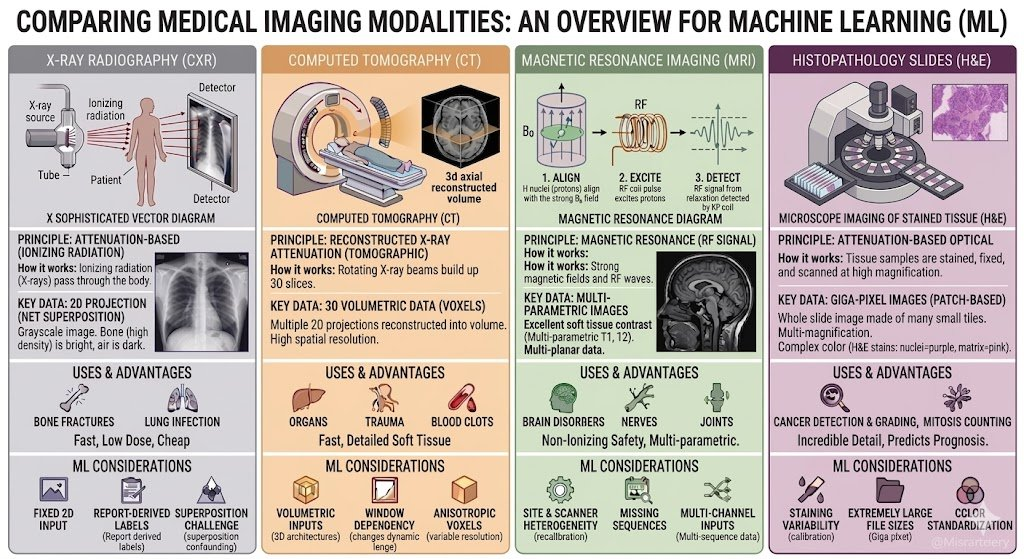
\includegraphics[width=\textwidth,height=0.78\textheight,keepaspectratio]{infographic1_core.png}
\end{center}
\end{frame}

% ============================================================


% ============================================================
\begin{frame}{Real Medical Images Across Modalities}
\begin{center}
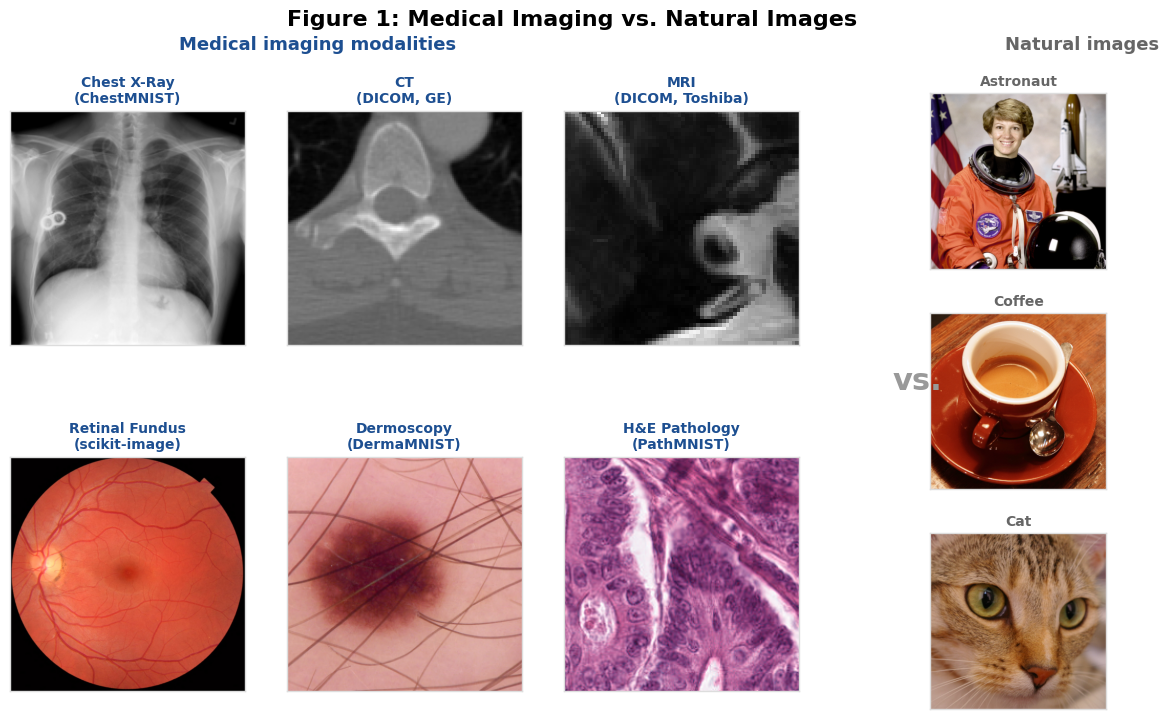
\includegraphics[width=\textwidth,height=0.70\textheight,keepaspectratio]{fig1_visual_survey.png}
\end{center}
\vspace{-0.5em}
{\scriptsize Top: real chest X-ray (ChestMNIST), CT (pydicom), MRI (pydicom), retinal fundus (scikit-image). Bottom: dermoscopy (DermaMNIST), H\&E pathology (PathMNIST), and natural images for comparison.}
\end{frame}

% ============================================================
\begin{frame}{How Imaging Enters Clinical Care}
\begin{center}
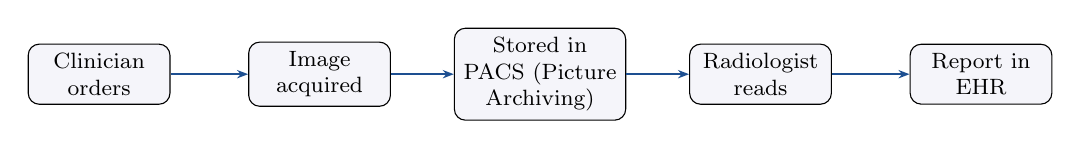
\begin{tikzpicture}[
    box/.style={draw, rounded corners, minimum width=1.8cm, minimum height=0.6cm,
                align=center, font=\footnotesize, fill=softbg},
    arr/.style={-{Stealth[length=4pt]}, thick, columbia}
]
\node[box] (order) at (0,0) {Clinician\\orders};
\node[box] (acquire) at (2.8,0) {Image\\acquired};
\node[box] (pacs) at (5.6,0) {Stored in\\PACS (Picture\\Archiving)};
\node[box] (read) at (8.4,0) {Radiologist\\reads};
\node[box] (report) at (11.2,0) {Report in\\EHR};

\draw[arr] (order) -- (acquire);
\draw[arr] (acquire) -- (pacs);
\draw[arr] (pacs) -- (read);
\draw[arr] (read) -- (report);
\end{tikzpicture}
\end{center}

\vspace{0.3em}
\textbf{Recall L17 (EHR):} Each study is an \emph{event} in the patient timeline. The image lives in the \textbf{PACS} (Picture Archiving and Communication System)---dedicated software for storing and distributing medical images. Like EHR systems, PACS are often proprietary with vendor lock-in.

\vspace{0.3em}
\textbf{Recall L19 (Text):} The radiology report is the most common \emph{label source} for imaging ML. We'll see how NLP label extraction creates noise shortly.

\vspace{0.3em}
\pause
\textbf{New in this unit:} Images are the first \emph{regular-grid} data type---prior modalities (EHR events, text) were irregular sequences.
\end{frame}

% ============================================================
\section{2D Projection Imaging: X-Ray}
% ============================================================

\begin{frame}{How X-Rays Work}
\textbf{Projection imaging:} X-ray source emits photons through the body. Dense tissue absorbs more. A flat detector captures what remains $\to$ 2D image.

\vspace{0.3em}
\pause
\textbf{The key concept---superposition:} Unlike a photograph (closer objects \emph{block} farther ones), an X-ray \emph{sums everything} along the beam path. A lung nodule behind the heart may be invisible.

\vspace{0.3em}
\pause
\textbf{Why grayscale?} X-rays measure one quantity (absorption). No color---intensity directly encodes tissue density. Bone = bright, air = dark.

\vspace{0.3em}
\textbf{vs.\ photographs:} Photos capture \emph{reflected} light (RGB, surfaces). X-rays capture \emph{transmitted} radiation (1 channel, internal structure).
\end{frame}

% ============================================================
\begin{frame}{Example: A Real Chest X-Ray}
\begin{columns}[c]
\column{0.42\textwidth}
\begin{center}
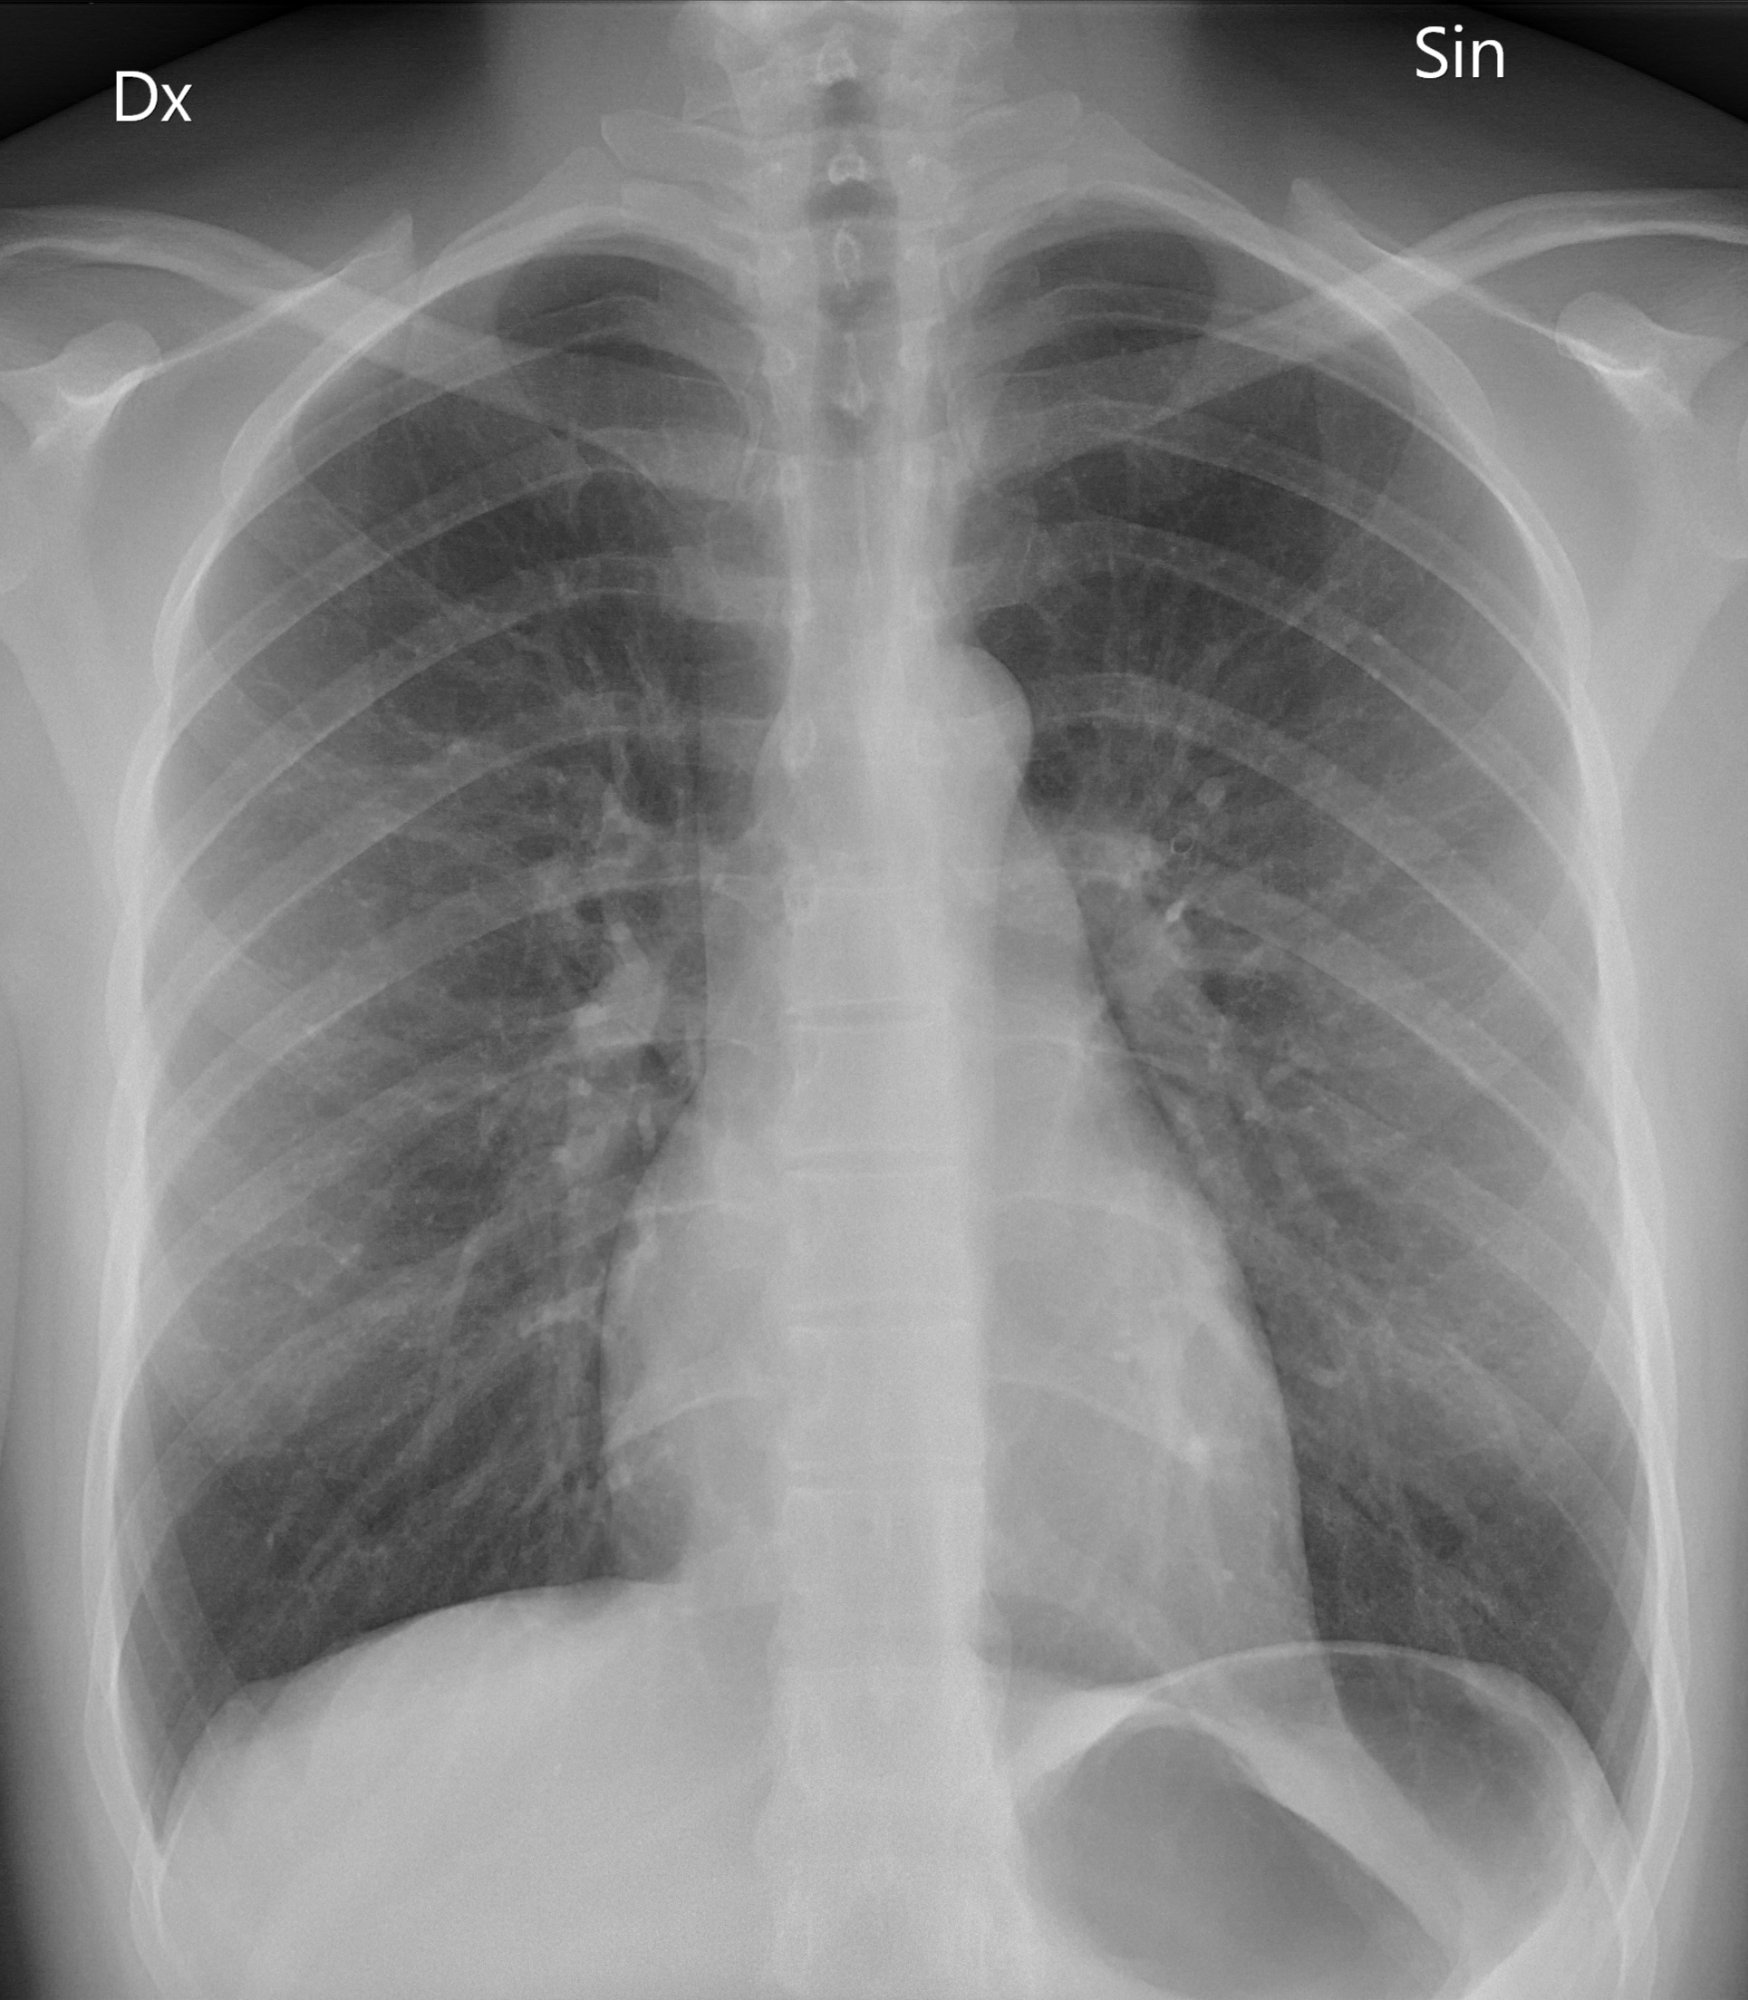
\includegraphics[width=\textwidth,height=0.70\textheight,keepaspectratio]{real_cxr.png}
\end{center}
\column{0.55\textwidth}
\textbf{What you see:}
\begin{itemize}
    \item Bright: ribs, spine, clavicles (bone absorbs X-rays)
    \item Dark: lung fields (air transmits X-rays)
    \item Intermediate: heart, mediastinum (soft tissue)
    \item Everything superimposed---no depth separation
\end{itemize}

\vspace{0.3em}
\textbf{Note the labels:} ``Dx'' = dexter (right), ``Sin'' = sinister (left). These are the \emph{patient's} right and left---mirrored from the viewer's perspective. Getting orientation wrong is a real clinical and ML error.
\end{columns}
\end{frame}

% ============================================================
\begin{frame}{Chest X-Rays vs.\ Natural Images}
\begin{center}
{\small
\renewcommand{\arraystretch}{1.2}
\begin{tabular}{p{2.5cm}p{4.2cm}p{4.5cm}}
\toprule
\textbf{Property} & \textbf{Natural Images} & \textbf{Chest X-Rays} \\
\midrule
Color & RGB (3 channels) & Grayscale (1 channel) \\
Depth & Closer objects \emph{block} farther ones & All depths \emph{summed} (superimposed) \\
Signal & Texture, color, shape & \emph{Intensity} is the signal \\
Findings & Large, salient objects & Subtle (3\,mm nodule = cancer) \\
Acquisition & Phone, varied & Standardized protocol \\
Variation & Scene, pose, illumination & Positioning, dose, manufacturer \\
\bottomrule
\end{tabular}
}
\end{center}

\pause
\begin{block}{Key Takeaway}
Techniques built for ImageNet need adaptation. Augmentation, preprocessing, and evaluation must respect the \emph{physics of acquisition}.
\end{block}
\end{frame}


% ============================================================
\begin{frame}{X-Ray: Technology, Economics, and Safety}
\begin{columns}[T]
\column{0.48\textwidth}
\textbf{Technology \& economics:}
\begin{itemize}
    \item Cost: \$100--300/study (cheapest modality)
    \item Equipment: \$50K--200K
    \item Seconds to acquire, minutes to read
    \item Available in virtually every clinic worldwide
    \item Portable units for bedside ICU imaging
\end{itemize}

\column{0.48\textwidth}
\textbf{Safety:}
\begin{itemize}
    \item Ionizing radiation: chest X-ray $\approx$~0.02\,mSv (very low; $\sim$3 days of background)
    \item Mammography $\approx$~0.4\,mSv
    \item ALARA principle: As Low As Reasonably Achievable
    \item No contrast needed for most studies
    \item Pregnancy screening required
\end{itemize}
\end{columns}

\vspace{0.3em}
\pause
\textbf{ML data:} Most \emph{abundant} imaging modality. Low cost $\to$ massive public datasets. But ``portable'' vs.\ ``upright'' come from different populations $\to$ confounding.
\end{frame}

% ============================================================
\begin{frame}{Chest X-Ray Datasets}
\begin{center}
{\small
\renewcommand{\arraystretch}{1.1}
\begin{tabular}{lrrp{4cm}}
\toprule
\textbf{Dataset} & \textbf{Images} & \textbf{Labels} & \textbf{Access} \\
\midrule
NIH ChestX-ray14 & 112,120 & 14 pathologies & Free (NIH Box) \\
CheXpert & 224,316 & 14 pathologies & Free (Stanford) \\
MIMIC-CXR & 377,110 & 14 pathologies & PhysioNet (credentialed) \\
PadChest & 160,868 & 174 labels & Free (BIMCV) \\
VinDr-CXR & 18,000 & 28 + bounding boxes & Free (Vingroup) \\
\bottomrule
\end{tabular}
}
\end{center}

\pause
\textbf{Common properties:}
\begin{itemize}
    \item Labels from reports via NLP (``silver standard'')---recall L19's negation challenges
    \item Multi-label: single image, multiple findings
    \item Extreme class imbalance: ``No Finding'' $\sim$50--60\%
\end{itemize}
\end{frame}


% ============================================================
\begin{frame}{Chest X-Ray Label Distribution (Real Data)}
\begin{center}
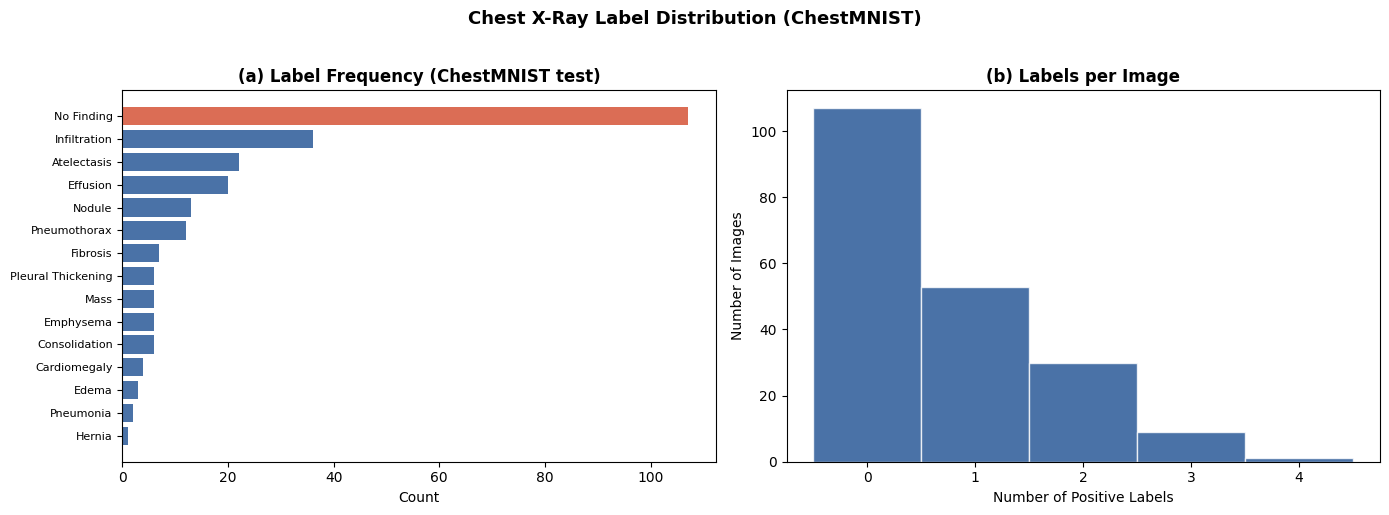
\includegraphics[width=\textwidth,height=0.75\textheight,keepaspectratio]{fig7_label_distribution.png}
\end{center}
\vspace{-0.3em}
{\small Real ChestMNIST data. Left: extreme class imbalance (``No Finding'' dominates). Right: most images have 0--1 positive labels; multi-label cases are rare but clinically important.}
\end{frame}

% ============================================================
\begin{frame}{Label Noise: The NLP Bottleneck}
{\small
\begin{center}
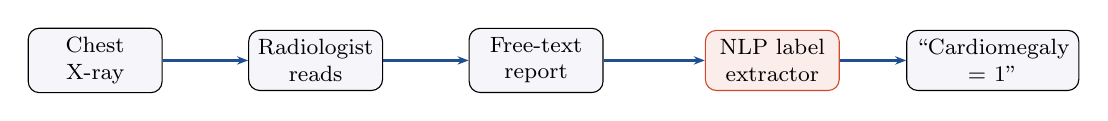
\begin{tikzpicture}[
    box/.style={draw, rounded corners, minimum width=1.7cm, minimum height=0.5cm,
                align=center, font=\footnotesize, fill=softbg},
    arr/.style={-{Stealth[length=4pt]}, thick, columbia}
]
\node[box] (img) at (0,0) {Chest\\X-ray};
\node[box] (rad) at (2.8,0) {Radiologist\\reads};
\node[box] (report) at (5.6,0) {Free-text\\report};
\node[box,fill=columbiaaccent!10,draw=columbiaaccent] (nlp) at (8.6,0) {NLP label\\extractor};
\node[box] (label) at (11.4,0) {``Cardiomegaly\\= 1''};

\draw[arr] (img) -- (rad);
\draw[arr] (rad) -- (report);
\draw[arr] (report) -- (nlp);
\draw[arr] (nlp) -- (label);
\end{tikzpicture}
\end{center}
}

\vspace{0.2em}
\textbf{Error sources (each adds noise):}
\begin{itemize}
    \item Radiologist miss rate ($\sim$3--5\% for subtle findings)
    \item Report ambiguity: ``cannot exclude pneumonia'' $\to$ positive or negative?
    \item NLP extraction: $\sim$5--15\% label noise on top of clinical uncertainty
\end{itemize}

\alert{You are training on labels that are themselves model outputs.}

{\small \textbf{Recall L19:} CheXpert uses a rule-based NLP labeler; negation and uncertainty handling are the key design choices---exactly the NLP challenges we studied.}
\end{frame}


% ============================================================
\begin{frame}{What Labels Actually Exist?}
\textbf{Label granularity varies enormously:}

\begin{center}
{\small
\renewcommand{\arraystretch}{1.1}
\begin{tabular}{p{2.2cm}p{2.8cm}p{2.8cm}p{3.5cm}}
\toprule
\textbf{Level} & \textbf{Example} & \textbf{Source} & \textbf{Implication} \\
\midrule
Image-level & ``Cardiomegaly'' & NLP from report & Classification \\
Study-level & ``Normal exam'' & Radiologist sign-off & Multi-image aggregation \\
Region/box & Nodule bounding box & Expert annotation (\$\$\$) & Detection \\
Pixel-level & Tumor mask & Manual tracing (hours) & Segmentation \\
Patient-level & 5-year mortality & EHR linkage & Prognosis \\
\bottomrule
\end{tabular}
}
\end{center}

\pause
\textbf{Key insight:} Moving down $\to$ labels get more expensive but more useful. Most large datasets have \emph{only} image- or study-level labels. This is why weak supervision (Thursday's MIL) matters.
\end{frame}

% ============================================================
\section{Volumetric Imaging: CT \& MRI}
% ============================================================

\begin{frame}{Computed Tomography (CT): Physics}
\begin{columns}[T]
\column{0.52\textwidth}
\textbf{How CT works:}
\begin{itemize}
    \item X-ray source \emph{rotates} around the body
    \item Reconstruct cross-sectional \emph{slices}
    \item Stack of slices $\to$ 3D volume
    \item \textbf{Voxels} (3D pixels): $512{\times}512{\times}300$+
\end{itemize}

\vspace{0.2em}
\pause
\textbf{Hounsfield units (HU):}
\begin{itemize}
    \item Standardized intensity scale
    \item Air~$=$~$-$1000, Water~$=$~0, Bone~$\approx$~$+$1000
    \item \emph{Windowing}: map HU range to display
\end{itemize}

\column{0.45\textwidth}
\begin{center}
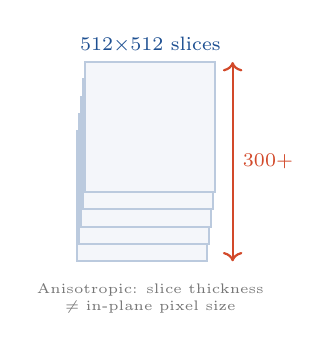
\begin{tikzpicture}[scale=0.55]
    \foreach \i in {0,0.4,0.8,1.2,1.6} {
        \draw[thick,fill=columbia!5,draw=columbia!30]
            (0+\i*0.12,\i) rectangle (3+\i*0.12,3+\i);
    }
    \node[font=\scriptsize,columbia] at (1.7, 5.0) {$512{\times}512$ slices};
    \draw[<->,thick,columbiaaccent] (3.6,0) -- (3.6,4.6)
        node[midway,right,font=\scriptsize] {300+};
    \node[font=\tiny,below,align=center,columbiagray] at (1.7,-0.3)
        {Anisotropic: slice thickness\\$\neq$ in-plane pixel size};
\end{tikzpicture}
\end{center}
\end{columns}
\end{frame}

% ============================================================
\begin{frame}{CT: Scrolling Through a Volume}
\begin{center}
% Animation plays in Okular, Acrobat, Foxit. Shows first frame in other viewers.
\animategraphics[autoplay,loop,width=0.50\textwidth]{8}{figures/ct_frames_small/ct_frame_}{000}{029}
\end{center}
\vspace{-0.3em}
\textbf{The key difference from X-ray:} CT gives you a full 3D volume. Scroll slice by slice---nothing is hidden behind anything else.

\vspace{0.2em}
{\small Animation: open PDF in \textbf{Okular} (Linux), Acrobat, or Foxit. Backup: open \texttt{figures/CT.gif} directly.}
\end{frame}

% ============================================================
\begin{frame}{CT: Windowing Matters}
\textbf{Same data, different windows.} W (width) and L (level/center) define which HU range is visible. Everything outside clips to black or white.

\begin{center}
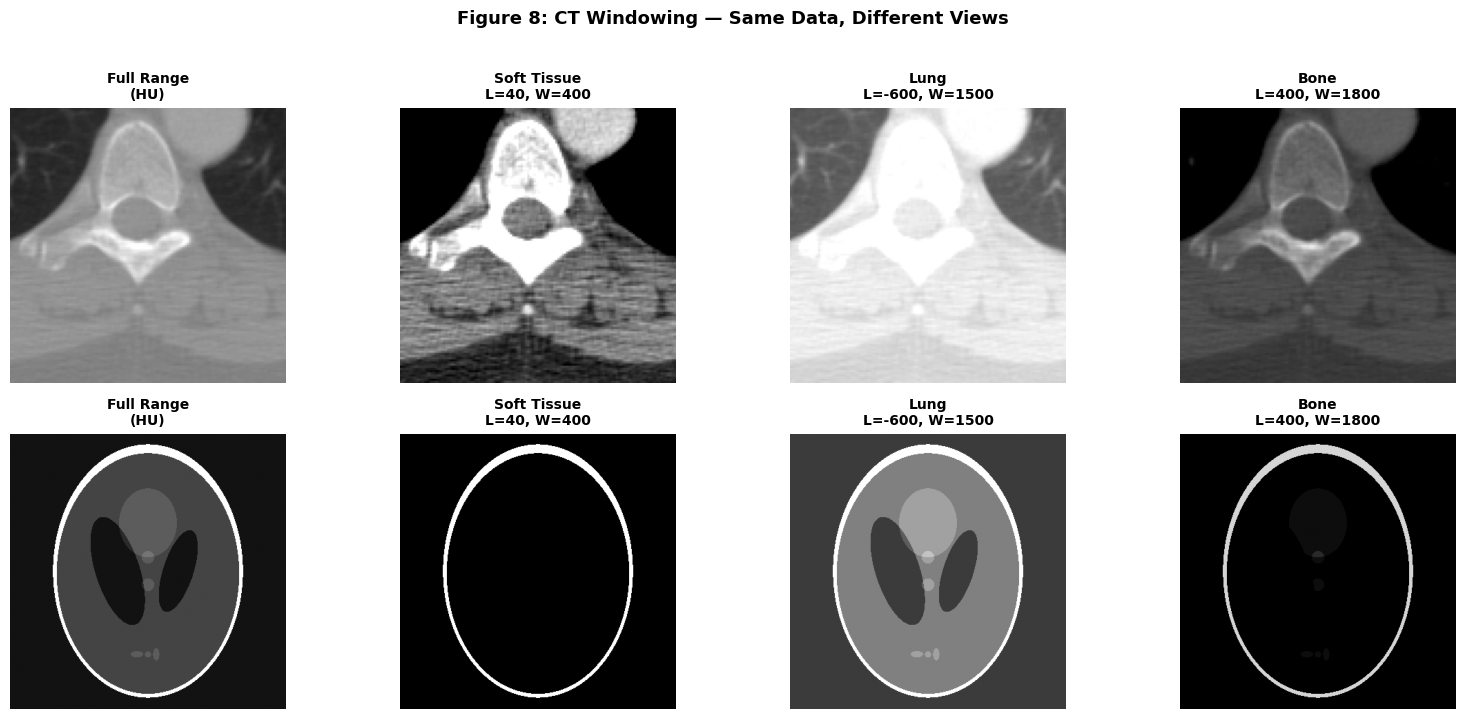
\includegraphics[width=\textwidth,height=0.55\textheight,keepaspectratio]{fig8_ct_windowing_real.png}
\end{center}
\vspace{-0.3em}
{\scriptsize Real pydicom CT test image under four window settings. See notebook Fig.~8.}
\pause
\textbf{Why this matters:} Raw HU gives low contrast for any single tissue. Common strategy: stack windows as channels (lung + soft + bone $\to$ 3-channel input, analogous to RGB).
\end{frame}

% ============================================================
\begin{frame}{CT: Technology, Economics, and Safety}
\begin{columns}[T]
\column{0.48\textwidth}
\textbf{Technology \& economics:}
\begin{itemize}
    \item Cost: \$500--3{,}000/study
    \item Equipment: \$1--2M per scanner
    \item Speed: full chest CT in $<$1\,s
    \item Common in EDs (trauma, stroke, PE)
\end{itemize}

\column{0.48\textwidth}
\textbf{Safety:}
\begin{itemize}
    \item \alert{Significant radiation:} chest CT $\approx$~2--7\,mSv
    \item Abdominal CT $\approx$~10--20\,mSv (denser tissue)
    \item Iodinated contrast: allergy, kidney risk
    \item Cumulative dose concern (pediatrics)
\end{itemize}
\end{columns}

\vspace{0.3em}
\pause
\textbf{ML data:} Abundant in high-income settings, sparse in low-resource. Most public datasets from a few academic centers $\to$ geographic bias.
\end{frame}

% ============================================================
\begin{frame}{MRI: What ML Practitioners Need to Know}
\textbf{Key advantage:} No ionizing radiation. Excellent soft tissue contrast. The dominant modality for brain, spine, joints, and cardiac imaging.

\vspace{0.3em}
\textbf{The critical ML difference from CT:} MRI can produce \emph{multiple images} of the same anatomy, each emphasizing different tissue properties (called ``sequences''). Same patient, same scan session, but the images look completely different.

\vspace{0.3em}
\pause
\textbf{Three ML challenges unique to MRI:}
\begin{enumerate}
    \item \alert{No standardized intensity scale.} Unlike CT (water=0\,HU everywhere), MRI signal depends on scanner hardware, field strength, and protocol. The same tissue produces different numbers on different machines.
    \item \textbf{Variable multi-channel input.} Which sequences are acquired depends on the clinical question (e.g.\ brain tumor workup: 6 sequences; routine scan: 2). Your model must handle variable-size input.
    \item \textbf{Slow acquisition} (30--90\,min) $\to$ motion artifacts are common.
\end{enumerate}

{\small Because of \#1, models trained at one hospital often show degraded performance at another---the \emph{scanner} looks different, not the disease. This is the ``multi-site generalization'' problem.}
\end{frame}

% ============================================================
\begin{frame}{MRI: Scrolling Through a Brain Volume}
\begin{center}
\animategraphics[autoplay,loop,width=0.35\textwidth]{8}{figures/mri_frames_small/mri_frame_}{000}{029}
\end{center}
\vspace{-0.3em}
Like CT, MRI produces a 3D volume. But unlike CT, MRI can produce \emph{multiple different volumes} of the same anatomy, and the intensity values are \emph{not standardized} across scanners.

\vspace{0.2em}
{\small Animation: open in \textbf{Okular}. Backup: \texttt{figures/brain\_mri.gif}. Real brain MRI: $256{\times}256{\times}180$ voxels.}
\end{frame}

% ============================================================
\begin{frame}{MRI: Technology, Economics, and Safety}
\begin{columns}[T]
\column{0.48\textwidth}
\textbf{Technology \& economics:}
\begin{itemize}
    \item Cost: \$1K--5K+/study
    \item Equipment: \$1--3M+ (shielded room)
    \item Slow: 30--90\,min per session
    \item Throughput: 8--12 patients/day
\end{itemize}

\column{0.48\textwidth}
\textbf{Safety:}
\begin{itemize}
    \item \textbf{No ionizing radiation} (major advantage)
    \item Contraindicated with some metal implants
    \item Contrast agent risks (rare)
    \item Claustrophobia ($\sim$5--10\% intolerant)
\end{itemize}
\end{columns}

\vspace{0.3em}
\pause
\textbf{ML data implication:} Expensive $\to$ small datasets. No standard intensity $\to$ models that work at Hospital A often underperform at Hospital B. ``Harmonization'' is an active research area.
\end{frame}

% ============================================================
\begin{frame}{Volumetric Data: A Fundamental Shift from 2D}
\textbf{The key difference from photos and X-rays:} CT and MRI produce 3D volumes. You can ``scroll through'' the body slice by slice---nothing is hidden behind anything else.

\vspace{0.3em}
\pause
\textbf{But 3D data creates new ML challenges:}
\begin{itemize}
    \item \textbf{Anisotropic voxels:} Slice thickness (e.g.\ 5\,mm) $\neq$ in-plane resolution (e.g.\ 0.5\,mm). This means a standard 3D convolution kernel ``sees'' different physical distances in different directions---like using a ruler where each tick mark is a different length on each axis.
    \item \textbf{Variable size:} One CT might be $512{\times}512{\times}300$; another $512{\times}512{\times}150$
    \item \textbf{Memory:} A single volume is $\sim$150\,MB---cannot batch like $224{\times}224$ images
\end{itemize}

\vspace{0.2em}
\pause
\textbf{Common approaches:} Resample to isotropic voxels, crop/pad to fixed size, or process slice-by-slice. Each choice discards information. 3D convolutions work but are expensive.

\end{frame}

% ============================================================
\section{Histopathology}
% ============================================================

\begin{frame}{Histopathology: The Gigapixel Problem}
\begin{columns}[T]
\column{0.53\textwidth}
\textbf{Whole-slide images (WSI):}
\begin{itemize}
    \item Tissue on glass, stained with H\&E
    \item Scanned at 20--40$\times$ magnification
    \item $\sim$100K $\times$ 100K px ($\sim$10 gigapixels)
    \item \alert{Cannot fit in GPU memory}
\end{itemize}

\vspace{0.2em}
\pause
\textbf{Tile-based processing:}
\begin{itemize}
    \item Extract $256{\times}256$ patches at $20\times$
    \item Encode tiles with feature extractor
    \item Aggregate $\to$ slide-level prediction
\end{itemize}

\column{0.44\textwidth}
\begin{center}
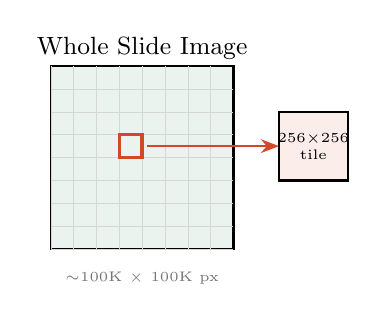
\begin{tikzpicture}[scale=0.58]
    \draw[thick,fill=hlgreen!10] (0,0) rectangle (4,4);
    \node[font=\small] at (2,4.4) {Whole Slide Image};
    \foreach \x in {0,0.5,...,3.5} {
        \draw[very thin, columbiagray!30] (\x,0) -- (\x,4);
    }
    \foreach \y in {0,0.5,...,3.5} {
        \draw[very thin, columbiagray!30] (0,\y) -- (4,\y);
    }
    \draw[very thick,columbiaaccent] (1.5,2) rectangle (2,2.5);
    \draw[-{Stealth},thick,columbiaaccent] (2.1,2.25) -- (5,2.25);
    \draw[thick,fill=columbiaaccent!10] (5,1.5) rectangle (6.5,3);
    \node[font=\tiny,align=center] at (5.75,2.25) {$256{\times}256$\\tile};
    \node[below,font=\tiny,columbiagray] at (2,-0.3) {$\sim$100K $\times$ 100K px};
\end{tikzpicture}
\end{center}
\end{columns}
\end{frame}

% ============================================================
\begin{frame}{Histopathology: Multi-Scale \& Staining}
\begin{center}
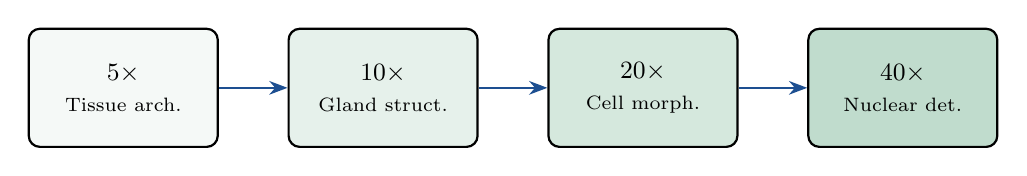
\begin{tikzpicture}[
    magbox/.style={draw, thick, rounded corners, minimum width=2.4cm,
                   minimum height=1.5cm, align=center, font=\small}
]
\node[magbox, fill=hlgreen!5] (m5) at (0,0) {$5\times$\\{\scriptsize Tissue arch.}};
\node[magbox, fill=hlgreen!12] (m10) at (3.3,0) {$10\times$\\{\scriptsize Gland struct.}};
\node[magbox, fill=hlgreen!20] (m20) at (6.6,0) {$20\times$\\{\scriptsize Cell morph.}};
\node[magbox, fill=hlgreen!30] (m40) at (9.9,0) {$40\times$\\{\scriptsize Nuclear det.}};

\draw[-{Stealth},thick,columbia] (m5) -- (m10);
\draw[-{Stealth},thick,columbia] (m10) -- (m20);
\draw[-{Stealth},thick,columbia] (m20) -- (m40);
\end{tikzpicture}
\end{center}

\vspace{0.3em}
Different tasks need different scales. Pathologists zoom in/out---models must too.

\vspace{0.3em}
\textbf{H\&E staining:} Hematoxylin (blue $\to$ nuclei) + Eosin (pink $\to$ cytoplasm). Color varies across labs $\to$ \emph{stain normalization} is critical preprocessing.

\vspace{0.3em}
\pause
\textbf{Weak supervision challenge:} Slide-level labels (from reports), not tile-level. A positive diagnosis may come from one small region in 10{,}000+ tiles. \alert{Formalized as Multi-Instance Learning on Thursday.}
\end{frame}

% ============================================================
\begin{frame}{Multi-Scale: Real H\&E Pathology}
\begin{center}
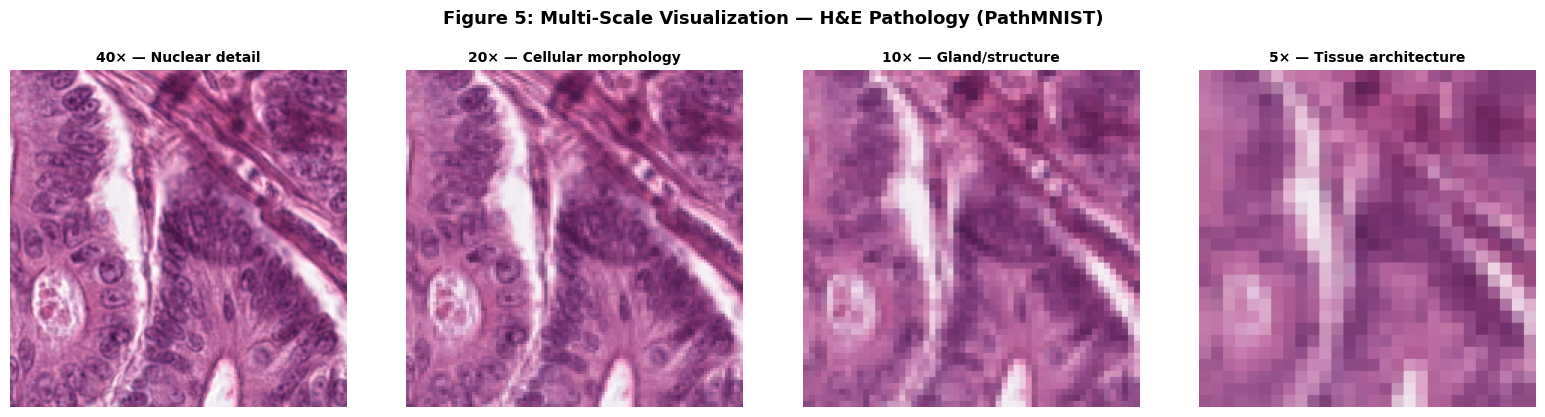
\includegraphics[width=\textwidth,height=0.75\textheight,keepaspectratio]{fig5_multiscale_pathology.png}
\end{center}
\vspace{-0.3em}
{\small Real H\&E pathology tissue (PathMNIST), downsampled to simulate 5$\times$--40$\times$ magnification. At 5$\times$ you see tissue architecture; at 40$\times$, individual cells (small round structures) and their nuclei (dark dots inside---stained purple by hematoxylin).}
\end{frame}

% ============================================================
\begin{frame}{Histopathology: Technology, Economics, and Access}
\begin{columns}[T]
\column{0.48\textwidth}
\textbf{Technology pipeline:}
\begin{itemize}
    \item Biopsy (invasive) $\to$ fix $\to$ section $\to$ stain $\to$ scan
    \item Scanner: \$100K--500K
    \item Scan: 1--5\,min/slide at 40$\times$
    \item Storage: 1--5\,GB/slide
    \item Digital adoption still incomplete worldwide
\end{itemize}

\column{0.48\textwidth}
\textbf{Economics \& access:}
\begin{itemize}
    \item TCGA: 30{,}000+ public slides
    \item Most pathology still on glass
    \item Labs scan selectively $\to$ bias
    \item No patient radiation risk
    \item FDA digital path clearance: 2017
\end{itemize}
\end{columns}

\vspace{0.3em}
\pause
\textbf{ML data:} Heavily biased toward academic cancer centers. Community hospital pathology differs in staining, scanners, demographics.
\end{frame}

% ============================================================
\section{Other Imaging Modalities}
% ============================================================

\begin{frame}{Other Modalities at a Glance}
{\small Retinal fundus, dermoscopy, ultrasound, and PET---each with distinct data properties and ML challenges:}
\begin{center}
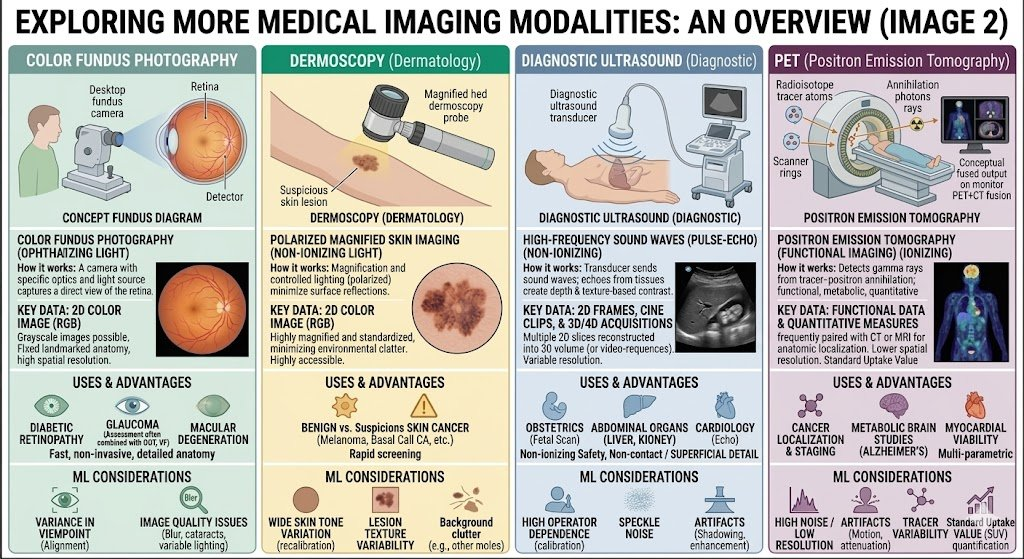
\includegraphics[width=\textwidth,height=0.78\textheight,keepaspectratio]{infographic2_other.png}
\end{center}
\end{frame}

% ============================================================
\begin{frame}{The Economics Shape the Data}
\begin{center}
{\footnotesize
\renewcommand{\arraystretch}{1.15}
\begin{tabular}{p{1.8cm}rp{1.8cm}p{2cm}p{2.8cm}}
\toprule
\textbf{Modality} & \textbf{Cost} & \textbf{Public data} & \textbf{Where} & \textbf{Bias risk} \\
\midrule
X-ray & \$100--300 & Massive & Global & Portable vs.\ upright \\
CT & \$500--3K & Large & High-income & Academic centers \\
MRI & \$1K--5K & Moderate & High-income & Scanner heterogeneity \\
Histopath. & Varies & Growing & Digitized labs & Cancer center bias \\
Retinal & \$30--100 & Large & Very broad & Camera quality \\
Derm. & \$50--200 & Large & Broad & \alert{Skin tone bias} \\
Ultrasound & \$200--500 & Small & Global & Operator skill \\
PET & \$3K--6K & Very small & Major ctrs & Wealth/geography \\
\bottomrule
\end{tabular}
}
\end{center}

\vspace{0.2em}
\pause
Cheaper modalities $\to$ larger datasets $\to$ more ML research $\to$ models that work best for populations already best served. \alert{Health equity concern.}
\end{frame}

% ============================================================
\begin{frame}{Radiation Dose Comparison}
\begin{center}
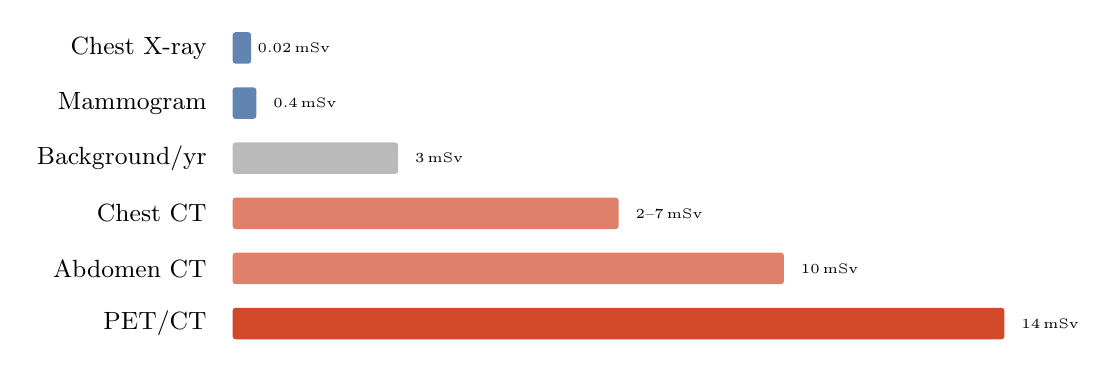
\begin{tikzpicture}[
    bar/.style={fill=columbia!70, minimum height=0.4cm, anchor=west, rounded corners=1pt},
    lbl/.style={font=\small, anchor=east}
]
\node[lbl] at (-0.2, 3.5) {Chest X-ray};
\node[bar, minimum width=0.06cm] at (0, 3.5) {};
\node[font=\tiny, anchor=west] at (0.2, 3.5) {0.02\,mSv};

\node[lbl] at (-0.2, 2.8) {Mammogram};
\node[bar, minimum width=0.3cm] at (0, 2.8) {};
\node[font=\tiny, anchor=west] at (0.4, 2.8) {0.4\,mSv};

\node[lbl] at (-0.2, 2.1) {Background/yr};
\node[bar, fill=columbiagray!50, minimum width=2.1cm] at (0, 2.1) {};
\node[font=\tiny, anchor=west] at (2.2, 2.1) {3\,mSv};

\node[lbl] at (-0.2, 1.4) {Chest CT};
\node[bar, fill=columbiaaccent!70, minimum width=4.9cm] at (0, 1.4) {};
\node[font=\tiny, anchor=west] at (5.0, 1.4) {2--7\,mSv};

\node[lbl] at (-0.2, 0.7) {Abdomen CT};
\node[bar, fill=columbiaaccent!70, minimum width=7.0cm] at (0, 0.7) {};
\node[font=\tiny, anchor=west] at (7.1, 0.7) {10\,mSv};

\node[lbl] at (-0.2, 0.0) {PET/CT};
\node[bar, fill=columbiaaccent, minimum width=9.8cm] at (0, 0.0) {};
\node[font=\tiny, anchor=west] at (9.9, 0.0) {14\,mSv};
\end{tikzpicture}
\end{center}

\vspace{0.2em}
\pause
You cannot collect CT/PET data ``just for research''---real radiation cost constrains dataset size and makes prospective collection ethically complex.

\vspace{0.1em}
{\small Retinal, dermoscopy, ultrasound, MRI: zero ionizing radiation.}
\end{frame}

% ============================================================
\section{DICOM \& Metadata}
% ============================================================

\begin{frame}{DICOM: The Universal Standard}
\textbf{DICOM} (Digital Imaging and Communications in Medicine):
\begin{itemize}
    \item Virtually all clinical images---X-ray, CT, MRI, ultrasound, PET---are stored in DICOM format
    \item Not just pixels---rich \textbf{metadata} in each file
\end{itemize}

\vspace{0.2em}
\begin{columns}[T]
\column{0.48\textwidth}
\textbf{Metadata for ML:}
\begin{itemize}
    \item Patient orientation (L/R, A/P)
    \item Pixel spacing (mm/pixel)
    \item Slice thickness (CT/MRI)
    \item Window center / width
    \item Manufacturer / scanner model
\end{itemize}

\column{0.48\textwidth}
\textbf{Why it matters:}
\begin{itemize}
    \item Pixel spacing varies $\to$ different scales
    \item Window/level changes visibility
    \item Manufacturer = distribution shift
    \item Must normalize in preprocessing
\end{itemize}
\end{columns}

\vspace{0.2em}
\pause
{\small Just as ICD/LOINC standardize EHR events (L17), DICOM standardizes imaging. Ignoring metadata is a common source of bugs in imaging ML pipelines.}
\end{frame}

% ============================================================
\begin{frame}{Real DICOM Metadata: Why It Matters}
\begin{center}
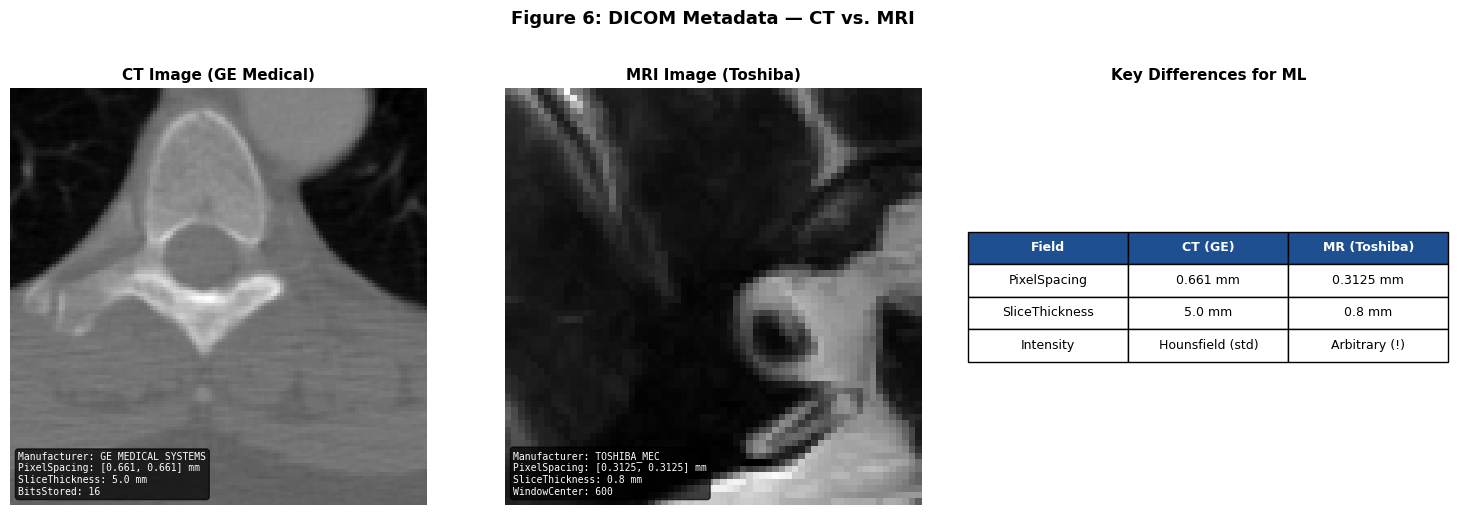
\includegraphics[width=0.85\textwidth,height=0.68\textheight,keepaspectratio]{fig6_dicom_metadata.png}
\end{center}
\vspace{-0.3em}
{\small Real CT (GE) and MRI (Toshiba) DICOM test files with metadata overlay, plus a key differences table. Different pixel spacings, intensity scales, and scanner models create distribution shift across sites.}
\end{frame}

% ============================================================
\begin{frame}{Accessing Medical Imaging Data}
\textbf{How do researchers actually get imaging data?}
\begin{enumerate}
    \item \textbf{Public datasets:} NIH, Stanford, PhysioNet release de-identified collections (see CXR table). Require varying levels of credentialing.
    \item \textbf{Institutional data:} Requires IRB approval, data use agreements (DUAs), and often months of negotiation
    \pause
    \item \textbf{De-identification:} DICOM headers contain PHI (name, DOB, MRN). Must be stripped. But images themselves can leak identity---CT facial reconstructions, dental patterns in panoramic X-rays
    \item \textbf{Federated learning:} Train models across sites without sharing raw data---an active research area motivated by these barriers
\end{enumerate}

\vspace{0.2em}
\pause
\textbf{Key contrast with other modalities:} Images carry unique re-identification risks: CT scans enable facial reconstruction, dental patterns are identifiable in panoramic X-rays, and DICOM headers may retain PHI even after ``de-identification.'' These risks differ from---but are not necessarily greater than---those of clinical text (L19).
\end{frame}

% ============================================================
\section{Data Quality \& Pitfalls}
% ============================================================

\begin{frame}{The Shortcut Learning Problem}
\begin{block}{Problem}
Models predict from \emph{acquisition metadata}, not pathology.
\end{block}

\vspace{0.2em}
\begin{center}
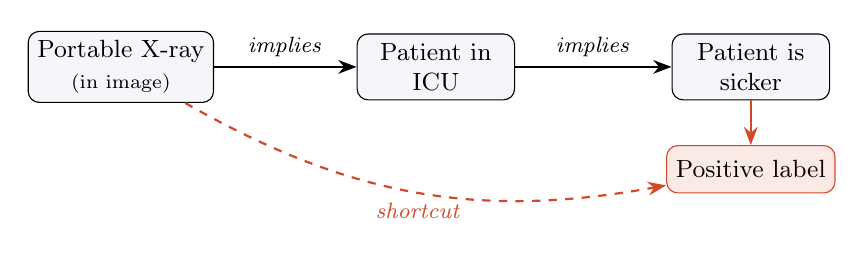
\begin{tikzpicture}[
    box/.style={draw, rounded corners, minimum width=2.0cm, minimum height=0.6cm,
                align=center, font=\small, fill=softbg},
    >=Stealth
]
\node[box] (port) at (0,0) {Portable X-ray\\{\scriptsize(in image)}};
\node[box] (icu) at (4,0) {Patient in\\ICU};
\node[box] (sick) at (8,0) {Patient is\\sicker};
\node[box,fill=columbiaaccent!12,draw=columbiaaccent] (label) at (8,-1.3) {Positive label};

\draw[->,thick] (port) -- node[above,font=\footnotesize] {\textit{implies}} (icu);
\draw[->,thick] (icu) -- node[above,font=\footnotesize] {\textit{implies}} (sick);
\draw[->,thick,columbiaaccent] (sick) -- (label);
\uncover<2->{\draw[->,thick,columbiaaccent,dashed] (port) to[bend right=20]
    node[below,font=\footnotesize\itshape,columbiaaccent] {shortcut} (label);}
\end{tikzpicture}
\end{center}

\vspace{0.2em}
\uncover<2->{High AUC from ``PORTABLE'' text, not pathology. Fails on external data.

\vspace{0.2em}
\alert{Recall Berkson's Paradox (L17):} conditioning on hospitalization creates spurious correlations. Here, conditioning on ``has a chest X-ray'' links acquisition type to disease severity---the model exploits the link instead of learning pathology.}
\end{frame}


% ============================================================


% ============================================================
\section{Summary \& Preview}
% ============================================================


% ============================================================
\begin{frame}{When You Encounter a New Imaging Dataset}
\textbf{Your five-question checklist} (reusable on any modality):

\vspace{0.3em}
\begin{enumerate}
    \item \textbf{Physics:} What physical signal does this image represent? Is it a projection, a volume, a time series? What does intensity \emph{mean}?
    \pause
    \item \textbf{Acquisition:} How much does it cost? Who gets scanned? Is there radiation? How does this shape who is in the dataset?
    \pause
    \item \textbf{Metadata:} What DICOM fields matter? Pixel spacing? Window settings? Scanner manufacturer? Have you normalized for these?
    \pause
    \item \textbf{Labels:} Where do labels come from---NLP, expert annotation, EHR linkage? At what level---image, study, pixel, patient? How noisy are they?
    \pause
    \item \textbf{Pitfalls:} What shortcuts could the model exploit? What distribution shifts will it face at deployment? What augmentations are safe?
\end{enumerate}

\vspace{0.2em}
\textbf{Thursday:} How to \emph{model} this data---transfer learning, U-Net, \alert{MIL}, foundation models.
\end{frame}

% ============================================================
\begin{frame}{End-to-End: One Chest X-Ray Study}
\textbf{Applying the five questions to a single imaging event:}

\vspace{0.2em}
\begin{enumerate}
    \item \textbf{Physics:} X-ray attenuation, 2D superposition
    \item \textbf{Acquisition:} Portable AP in ICU, \$150, 0.02\,mSv radiation
    \item \textbf{Metadata:} DICOM says ``PORTABLE,'' 0.14\,mm/px, GE scanner
    \item \textbf{Labels:} Report: ``bilateral opacities'' $\to$ NLP extracts Edema = 1
    \item \textbf{Pitfall:} Model learns ``PORTABLE'' text $\to$ sick (shortcut!)
\end{enumerate}

\vspace{0.3em}
\pause
\textbf{What went wrong:} ``PORTABLE'' correlates with ICU patients (sicker). Model learns this shortcut $\to$ high internal AUC, fails on external data.

\vspace{0.2em}
\textbf{How you'd catch it:} Inspect DICOM metadata $\to$ notice correlation $\to$ test on non-portable subset $\to$ AUC drops. \alert{The framework predicts this failure.}

\vspace{0.1em}
{\small \textbf{Practical rule:} Always inspect your data. A 10-minute visual audit catches problems that waste weeks.}
\end{frame}

% ============================================================
\begin{frame}{Companion Notebook}
\textbf{\texttt{nb21\_medical\_imaging\_data.ipynb}} --- run to regenerate today's figures:
\begin{enumerate}
    \item Visual survey: medical vs.\ natural images
    \item Pixel intensity distributions per modality
    \item Pathology multi-scale visualization
    \item DICOM metadata comparison (CT vs.\ MRI)
    \item CT windowing under different W/L settings
    \item Label distribution \& class imbalance (ChestMNIST)
\end{enumerate}

\textbf{How to use:} Run all cells, then experiment---change augmentation parameters, zoom levels, or normalization. All outputs save to \texttt{figures/}.

\textbf{Thursday (L22):} Transfer learning, U-Net, \alert{MIL}, foundation models.
\end{frame}

% ============================================================
\begin{frame}[standout]
    Questions?
\end{frame}


% ============================================================
\appendix
% ============================================================

\begin{frame}{Appendix: Intensity Distributions by Modality}
\begin{center}
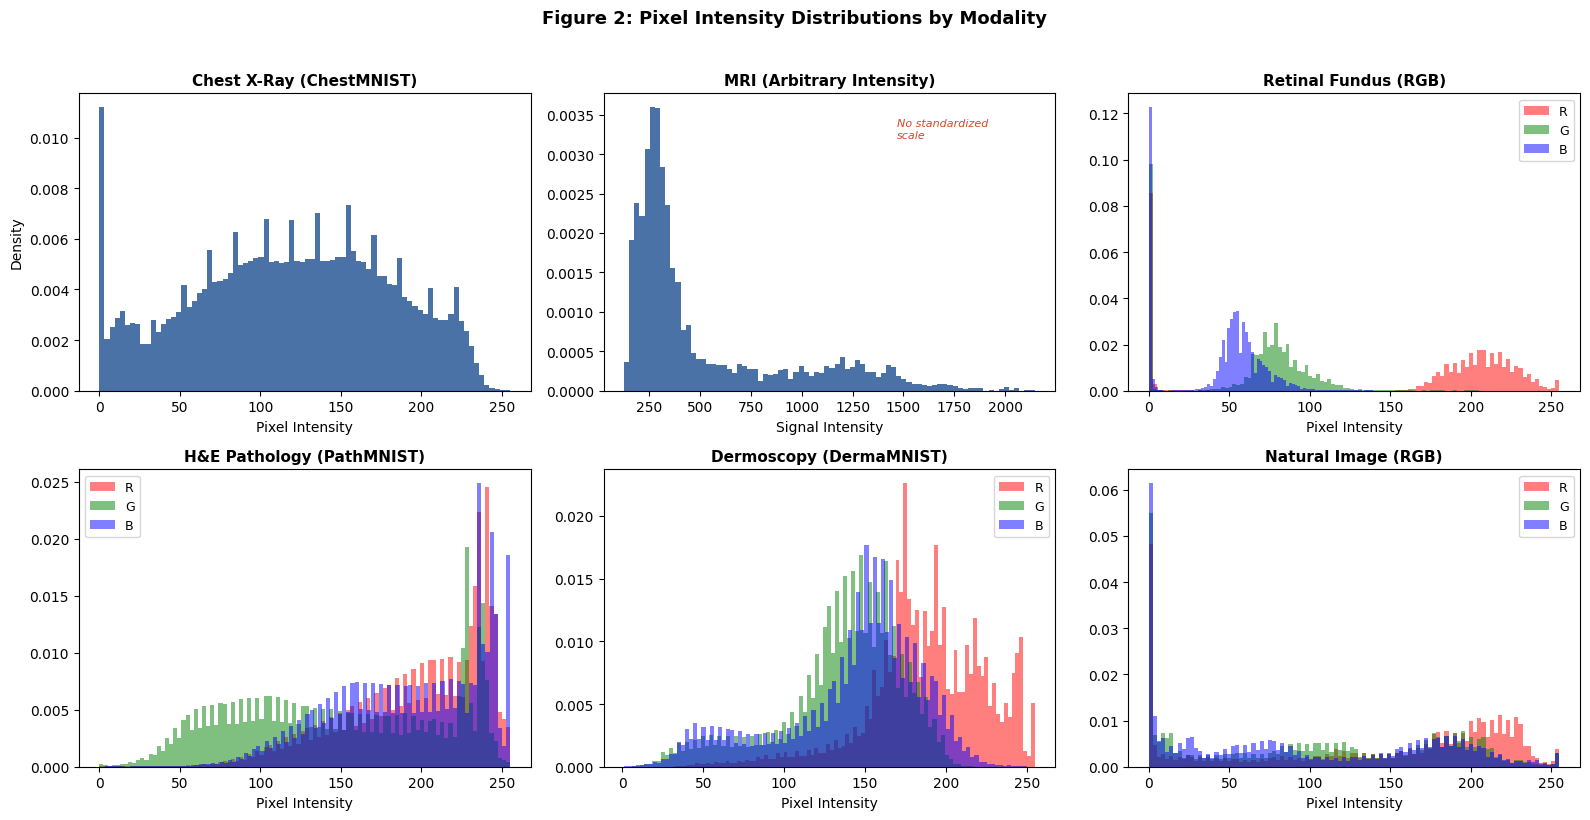
\includegraphics[width=\textwidth,height=0.75\textheight,keepaspectratio]{fig2_intensity_distributions.png}
\end{center}
\vspace{-0.3em}
{\small Chest X-ray, MRI, retinal, H\&E pathology, dermoscopy, and natural images. Each modality has a characteristic distribution. ImageNet normalization is inappropriate for most medical modalities. See notebook Fig.~2.}
\end{frame}

% ============================================================
\begin{frame}{Appendix: Frequency Content by Modality}
\begin{center}
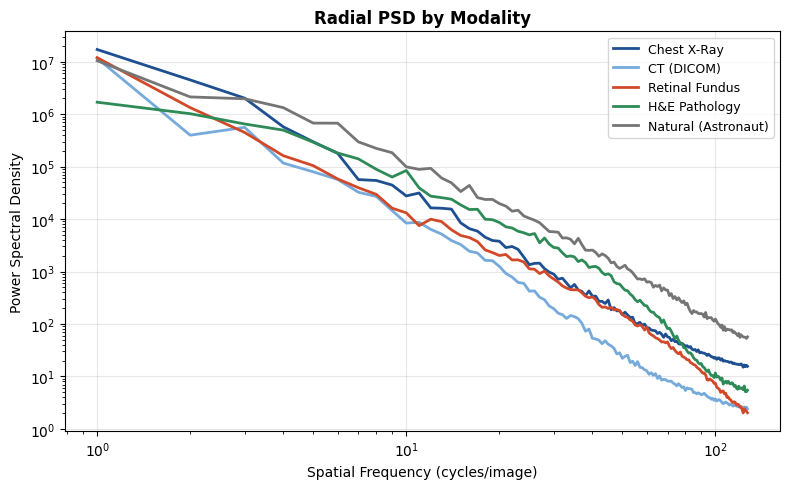
\includegraphics[width=\textwidth,height=0.75\textheight,keepaspectratio]{fig3_frequency_analysis.png}
\end{center}
\vspace{-0.3em}
{\small Medical images have more low-frequency energy and less high-frequency texture than natural images. Practically: ImageNet features may be less useful for smooth medical images. See notebook Fig.~3.}
\end{frame}


% ============================================================
\begin{frame}{Appendix: Even More Imaging Modalities}
\begin{center}
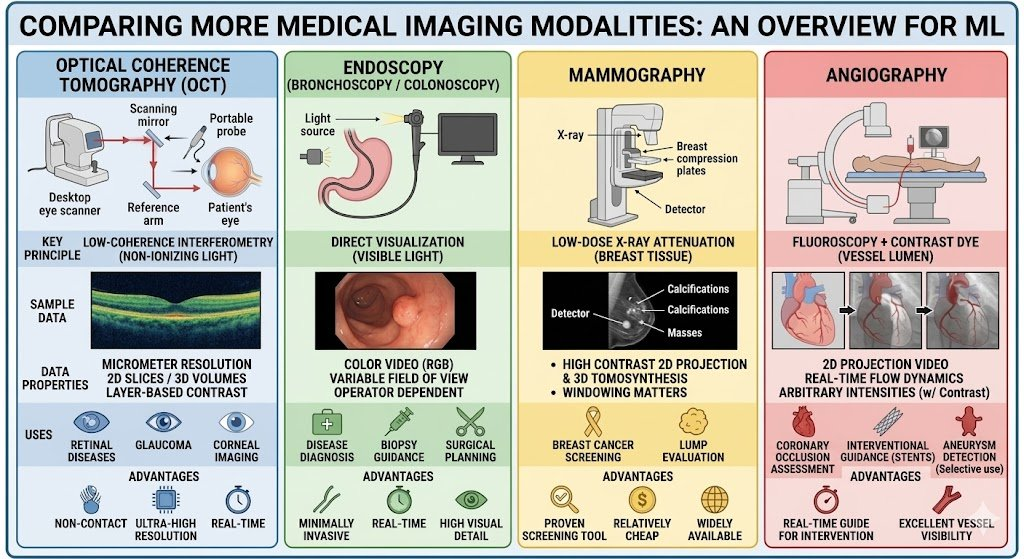
\includegraphics[width=\textwidth,height=0.80\textheight,keepaspectratio]{infographic3_more.png}
\end{center}
\vspace{-0.3em}
{\small OCT (retinal cross-sections), endoscopy (direct visualization), mammography (specialized X-ray), and angiography (vessel imaging). Each has distinct ML challenges.}
\end{frame}

\end{document}